\documentclass[11pt]{report}
%\usepackage[margin=0.75in]{geometry}
\usepackage{geometry}
\usepackage[utf8]{inputenc}
\usepackage[greek, spanish, es-tabla]{babel}
\usepackage[bottom]{footmisc}
\usepackage[tt]{titlepic}
\usepackage{url}
\usepackage{xurl}
\usepackage{graphicx}
\usepackage{makeidx}
\usepackage{enumerate}
\usepackage{fancyhdr, ragged2e}
\usepackage{eurosym}
\usepackage{float}
\usepackage{titlesec}
\usepackage[bookmarks,hidelinks]{hyperref}
\usepackage{nameref}
\usepackage{enumitem}
\usepackage{booktabs}
\usepackage[table]{xcolor}
\usepackage{multirow}
\usepackage{amsmath}
\usepackage{listings}
\usepackage{subcaption}

	%\addtolength{\oddsidemargin}{-.8in}
	%\addtolength{\evensidemargin}{-.8in}
	%\addtolength{\textwidth}{1.45in}

	\addtolength{\topmargin}{-.1in}
	\addtolength{\textheight}{1.25in}

\graphicspath{{figures/}}
\pagestyle{fancy}
\renewcommand{\chaptermark}[1]{\markboth{\scriptsize\MakeUppercase{#1}}{}}
\renewcommand{\sectionmark}[1]{\markright{\tiny\MakeUppercase{#1}}{}}
\fancyfoot{}
%\fancyfoot[RO, LE] {\thepage}
\fancyfoot[R] {\thepage}
%\fancyfoot[LO, RE] {\scriptsize Escuela de Ingeniería Informática - Universidad de Oviedo. Mª Isabel Fernández Pérez}
\fancyfoot[L] {\scriptsize Escuela de Ingeniería Informática - Universidad de Oviedo. Mª Isabel Fernández Pérez}

\renewcommand{\footrulewidth}{0.4pt}
%Evita warnings de cabecera
\setlength{\headheight}{15pt}
\setcounter{secnumdepth}{4}

%Esto es para poder ponerle un formato bien hecho a los \paragraph{}
\titleformat{\paragraph}
{\normalfont\normalsize\bfseries}{\theparagraph}{1em}{}
\titlespacing*{\paragraph}
{0pt}{3.25ex plus 1ex minus .2ex}{1.5ex plus .2ex}

%Y esto para para ponerselo a los \subparagraph{}
\titleformat{\subparagraph}
{\normalfont\normalsize\bfseries}{\theparagraph}{1em}{}
\titlespacing*{\subparagraph}
{0pt}{1ex plus 1ex minus .2ex}{1.5ex plus .2ex}


\makeindex

\begin{document}
\selectlanguage{spanish} 

\hypersetup{pageanchor=false}
\begin{titlepage}
	\centering
	
\includegraphics[width=0.2\textwidth]{EscudoUniovi}
	\hspace{3 cm}
	
\includegraphics[width=0.3\textwidth]{EscudoEscuela}
	\par\vspace{1cm}
	
	\vspace{1.5cm}
	{\huge\bfseries Creación del sitio web para el Museo de la Informática de la Escuela de Ingeniería Informática de Oviedo\par}
	\vspace{2cm}
	{\large \textbf{GRADO EN INGENIERÍA INFORMÁTICA DEL SOFTWARE} \par}
	\vspace{1cm}
	{\scshape\Large Trabajo Fin de Grado\par}
	%\vfill
   	
  \vspace{2cm}
	%\vfill
	\textbf{AUTOR}\par
	 Mª Isabel Fernández Pérez \\
	%\vfill
	\vspace{1.5cm}
	%{\Large\itshape Mª Isabel Fernández Pérez\par}
	%\vfill
	\textbf{TUTOR}\par
	José Manuel Redondo López
	\vfill
	
	{\large Julio 2021 \par}
\end{titlepage}


\newpage
Copyright (C) 2020 \textbf{ELENA ALLEGUE GONZÁLEZ, JOSÉ MANUEL REDONDO LÓPEZ} \\
Teaching Innovation Project: PINN-19-A-029 (University of Oviedo)\\
This work has been published in \cite{RedondoPlantillasRG19} \cite{RedondoUCO20}\\
\\
Esta versión de la plantilla para Trabajos de Fin de Grado ha sido posible gracias a la donación de la ex-alumna Elena Allegue González de su documentación de Trabajo de Fin de Grado, que ha servido como base para elaborar esta versión. Aquí podréis encontrar todos los títulos y subtítulos de las secciones, pero las explicaciones se mantendrán en la versión \textit{Word} de la plantilla (se proporciona una versión PDF de la misma para facilitar el acceso a las mismas). No obstante, del trabajo de Elena se han conservado ejemplos de como hacer elementos clave como imágenes, tablas, etc.

Desarrollar una versión \textit{Latex} de la plantilla desde cero es una trabajo bastante largo, pero gracias al trabajo de Elena se ha podido equiparar esta versión con las de \textit{Word} mucho más rápidamente.

%\newpage
\thispagestyle{empty}
\chapter*{Agradecimientos}


\pagestyle{fancy}
\renewcommand{\chaptermark}[1]{\markboth{\scriptsize\MakeUppercase{#1}}{}}
\renewcommand{\sectionmark}[1]{\markright{\tiny\MakeUppercase{#1}}{}}

%\fancyhead{}
%\lhead{\parbox[t]{0.5\textwidth}{\RaggedRight\rightmark\strut}}
%\rhead{\parbox[t]{0.5\textwidth}{\RaggedLeft\leftmark\strut}}
%\setlength{\headheight}{5\baselineskip}

\fancyfoot{}
%\fancyfoot[RO, LE] {\thepage}
\fancyfoot[R] {\thepage}
%\fancyfoot[LO, RE] {\scriptsize Escuela de Ingeniería Informática - Universidad de Oviedo. Mª Isabel Fernández Pérez}
\fancyfoot[L] {\scriptsize Escuela de Ingeniería Informática - Universidad de Oviedo.  Mª Isabel Fernández Pérez}
\renewcommand{\footrulewidth}{0.4pt}
\pagenumbering{arabic}
%\newpage


\thispagestyle{empty}


\setcounter{tocdepth}{2}
\setcounter{secnumdepth}{4}
\pagestyle{empty}
{
  \renewcommand{\thispagestyle}[1]{}
  \tableofcontents
}
\clearpage


\newpage
{
  \renewcommand{\thispagestyle}[1]{}
  \listoffigures
}
\clearpage

\newpage
{
  \renewcommand{\thispagestyle}[1]{}
  \listoftables
}
\clearpage

\newpage
\hypersetup{pageanchor=true}

\newpage
\thispagestyle{empty}
\chapter{¿Qué es este trabajo?}
\section{Resumen}
El objetivo de este proyecto es crear el sitio web del Museo de la Informática de la Escuela de Ingeniería Informática, para exponer los componentes que están disponibles. Inicialmente se expondrán CPUs, pero está pensado para añadir en un futuro otros componentes como, por ejemplo, GPUs.\\
\par
El usuario podrá navegar por los diferentes periodos históricos en los que se agrupan los componentes, conocer efemérides tecnológicas de la época y otras curiosidades. De cada pieza podrá ver características, sistemas famosos que la utilizaban, imágenes y la ubicación en la que se encuentran físicamente.
\newpage
\section{Palabras Clave}
Museo de la Informática, sitio web, componentes, hardware.
\pagestyle{fancy}
\newpage
\section{Abstract}
The aim of this project is to create the Computer Museum's website for the Computer Science School, to exhibit the available components. Initially, there wiill only be CPUs, but different components, like GPUs, can be added in the future.\\
\par
The user will be able to visit the different historical periods  in which components are grouped, to know technological ephemerides of that time and other curiosities. For each piece, the user will also be able to see its characteristics, famous systems that used it and the location where they are physically located.
\pagestyle{fancy}
\newpage
\section{Keywords}
Computer Museum, website, components, hardware.

\pagestyle{fancy}
%\newpage
\chapter{PSI: PLANIFICACIÓN DEL SISTEMA DE INFORMACIÓN}

	\vspace{2cm}	
	\begin{center}
	{\Large \textbf{FASE DE PLANIFICACIÓN} \par}
	\end{center}
	\vspace{5cm}
	
	\begin{center}
	\Huge \textbf{PSI}\par
	\end{center}

\newpage

\section{PSI 1: INICIO DEL PLAN DE SISTEMAS DE INFORMACIÓN}

\subsection{PSI 1.1: Análisis de la Necesidad del PSI} 
El tutor de este trabajo de fin de grado, José Manuel Redondo, ha propuesto el desarrollo de una aplicación web para el Museo de la Informática de Asturias, que contenga toda la información disponible sobre los componentes del museo y la muestre de forma ordenada para que las personas interesadas puedan acceder a ella fácilmente. El sistema será gestionado directamente por el tutor del trabajo.\\
\par El sistema debe identificar cada componente, mostrar la información disponible del mismo, e indicar la localización física de cada uno para ofrecer la posibilidad de visitar presencialmente el lugar de exposición de este. El software permitirá añadir la información de las nuevas piezas que puedan ser incluidas en la exposición en un futuro gracias a donaciones o compras. Los componentes serán ordenados según su tipo y la época a la que pertenecen. Además, el sistema automatizará la creación de los carteles informativos que acompañan a los componentes en la exposición física del Museo. 

\newpage
\subsection{PSI 1.2: Identificación del Alcance del PSI}
Actualmente las piezas del museo se encuentran expuestas en la Escuela de Ingeniería Informática, acompañadas de los carteles informativos correspondientes. Los objetivos de este proyecto son los siguientes:
\begin{itemize}
	\item Recopilar los datos disponibles de las piezas que se encuentran actualmente en el Museo e introducirlos en una base de datos.	
	\item Mostrar una linea temporal con los diferentes periodos a los que pertenecen los componentes del Museo. 
	\item Permitir acceder a cada periodo para ver los componentes del mismo.
	\item Organizar las diferentes piezas en función de su tipo y de la familia de la que forman parte.
	\item Presentar la información disponible de cada pieza, así como imágenes de la misma y otras curiosidades.
	\item Automatizar la creación de los carteles, utilizando plantillas predefinidas que se rellenarían con la información y las fotografías disponibles de la familia de piezas pertinente, que hasta el momento se han realizado de forma manual con Microsoft Publisher.  De este modo, se facilitará la exposición de nuevas piezas, ya que el esfuerzo de crear cada cartel informativo se reducirá de forma considerable. Los carteles están organizados por familia de piezas, más concretamente por familias de CPU.
\end{itemize}
En definitiva, estos objetivos se pueden resumir en:
\begin{itemize}
	\item Permitir a los usuarios visitar el Museo de la Informática de forma online, ofreciendo la misma información que se encuentra disponible en la exposición física.
	\item Facilitar el proceso de exposición de nuevas piezas gracias a la creación automática de la cartelería.
\end{itemize}

\newpage
\subsection{PSI 1.3: Determinación de Responsables}
\begin{itemize}
	\item \textbf{El proyectante} se encargará del desarrollo del software descrito y de realizar la carga de los datos disponibles a la base de datos correspondientes.
	\item\textbf{El tutor del proyecto} se encargará de la supervisión de las fases del proyecto y de su validación.
	\item \textbf{Una serie de usuarios escogidos aleatoriamente} realizará pruebas del software para comprobar su correcto funcionamiento.
\end{itemize}

\newpage
\section{PSI 2: DEFINICIÓN Y ORGANIZACIÓN DEL PSI}
 

\subsection{PSI 2.1: Especificación del Ámbito y Alcance} 


\subsection{PSI 2.2: Organización del PSI}



\newpage
\section{PSI 3: ESTUDIO DE LA INFORMACIÓN RELEVANTE}
 
\subsection{PSI 3.1: Selección y Análisis de Antecedentes} 


%\newpage
\chapter{PSI 7: DEFINICIÓN DE LA ARQUITECTURA TECNOLÓGICA}
	\vspace{2cm}	
	\begin{center}
	{\Large \textbf{FASE DE PLANIFICACIÓN} \par}
	\end{center}
	\vspace{5cm}
	
	\begin{center}
	\Huge \textbf{PSI}\par
	\end{center}

\newpage

\section{PSI 7.1: Identificación de las Necesidades de Infraestructura Tecnológica} 

\newpage
\section{PSI 7.2: Selección de la Arquitectura Tecnológica} 

\newpage
\chapter{ESTUDIO DE VIABILIDAD DEL SISTEMA}
	\vspace{2cm}	
	\begin{center}
	{\Large \textbf{FASE DE DESARROLLO} \par}
	\end{center}
	\vspace{5cm}
	
	\begin{center}
	\Huge \textbf{EVS}\par
	\end{center}

\newpage


\section{EVS 4, 5, 6: ESTUDIO Y VALORACIÓN DE ALTERNATIVAS DE SOLUCIÓN. SELECCIÓN DE ALTERNATIVA FINAL}

\subsection{Evaluación de alternativas de desarrollo} 
\subsubsection{Node.js y JavaScript}
Node.js es un entorno de ejecución de JavaScript orientado a eventos asíncronos, en el que no hace falta ultilizar hilos. Utiliza un modelo de entrada y salida sin bloqueo, lo que asegura un rendimiento más eficiente de la aplicación y evita que se produzca una gran sobrecarga del lado del servidor. Por ello, es muy apropiado para desarrollar sistemas escalables\cite{NodeJS}.\\
\par JavaScript es uno de los lenguajes más populares actualmente. Está basado en el estándar ECMAScript. Se trata un lenguaje interpretado, se compila en tiempo de ejecución. Es orientado a objetos, débilmente tipado y dinámico\cite{JavaScript}.\\
\par Esta fue la primera opción barajada, ya que había utilizado anteriormente estas tecnologías y podría aprovechar este proyecto para profundizar en su aprendizaje.
\begin{figure}[H]
	\begin{subfigure}{0.5\textwidth}
	\centering
	
\includegraphics[scale=0.5]{nodejs}
	\end{subfigure}
	\begin{subfigure}{0.5\textwidth}
	\centering
	
\includegraphics[scale=2.1]{javascript}
	\end{subfigure}
	\caption{Logos de Node.js y JavaScript}
\end{figure}

\subsubsection{Angular y TypeScript}
La otra opción considerada fue Angular con TypeScript, debido a su popularidad. No había trabajado con ellas antes, y esta sería una buena oportunidad para conocerlas.\\
\par Angular es un framework desarrollado en TypeScript y utilizado habitualmente para crear aplicaciones de una sola página. Se basa en la utilización de componentes web reutilizables para crear aplicaciones web fácilmente escalables. Angular extiende la sintaxis de HTML y actualiza automáticamente el árbol DOM cuando el estado de un componente cambia. Cuenta con gran cantidad de librerías y es uno de los frameworks más utilizados en la industria actual\cite{Angular}.\\
\par TypeScript es un lenguaje de programación que extiende JavaScript añadiendo la definición de tipos estáticos. Al compilarlo se transforma en código JavaScript siguiendo todos los estándares, y puede ejecutarse en cualquier lugar que ejecute JavaScript\cite{TypeScript}.
\begin{figure}[H]
	\begin{subfigure}{0.5\textwidth}
	\centering
	
\includegraphics[scale=0.40]{angular}
	\end{subfigure}
	\begin{subfigure}{0.5\textwidth}
	\centering
	
\includegraphics[scale=0.15]{typescript}
	\end{subfigure}
	\caption {Logos de Angular y TypeScript}
\end{figure}
Ambas opciones son de código abierto, lo que me parece un punto positivo ya que, gracias a la colaboración de la comunidad, se consigue una alta calidad en el software. \\
\par Finalmente, me decidí por Angular y TypeScript, principalmente por la razón de aprender estas dos tecnologías tan importantes actualmente en el desarrollo de aplicaciones web.

\newpage
\chapter{PLANIFICACIÓN Y GESTIÓN DEL TFG}
\newpage

\newpage
\section{PLANIFICACIÓN DEL PROYECTO}

\subsection{Identificación de Interesados}


\subsection{OBS y PBS}


\subsection{Planificación Inicial. WBS}


\subsection{Riesgos}

\subsubsection{Plan de Gestión de Riesgos} 

\subsubsection{Identificación de Riesgos}

\subsubsection{Registro de Riesgos} 



\subsection{Presupuesto Inicial}

\subsubsection{Presupuesto de Costes}

\subsubsection{Presupuesto de Cliente} 


\newpage
\section{EJECUCIÓN DEL PROYECTO}

\subsection{Plan Seguimiento de Planificación}

\subsection{Bitácora de Incidencias del Proyecto}

\subsection{Riesgos}


\newpage
\section{CIERRE DEL PROYECTO}

\subsection{Planificación Final}

\subsection{Informe Final de Riesgos}

\subsection{Presupuesto Final de Costes}

\subsection{Informe de Lecciones Aprendidas}



\newpage
\chapter{ANÁLISIS DEL SISTEMA DE INFORMACIÓN}
	\vspace{2cm}	
	\begin{center}
	{\Large \textbf{FASE DE DESARROLLO} \par}
	\end{center}
	\vspace{5cm}
	
	\begin{center}
	\Huge \textbf{ASI}\par
	\end{center}

\newpage


\section{ASI 1: DEFINICIÓN DEL SISTEMA}

\subsection{Determinación del Alcance del Sistema}


\newpage
\section{ASI 2: ESTABLECIMIENTO DE REQUISITOS}

\newlist{myEnumIU}{enumerate}{4}
\setlist[myEnumIU,1]{label=\textbf{RIU-\arabic*.}}
\setlist[myEnumIU,2]{label*=\textbf{\arabic*.}}
\setlist[myEnumIU,3]{label*=\textbf{\arabic*.}}
\setlist[myEnumIU,4]{label*=\textbf{\arabic*.}}

\newlist{myEnumIH}{enumerate}{4}
\setlist[myEnumIH,1]{label=\textbf{RIH-\arabic*.}}
\setlist[myEnumIH,2]{label*=\textbf{\arabic*.}}
\setlist[myEnumIH,3]{label*=\textbf{\arabic*.}}
\setlist[myEnumIH,4]{label*=\textbf{\arabic*.}}

\newlist{myEnumIC}{enumerate}{4}
\setlist[myEnumIC,1]{label=\textbf{RIC-\arabic*.}}
\setlist[myEnumIC,2]{label*=\textbf{\arabic*.}}
\setlist[myEnumIC,3]{label*=\textbf{\arabic*.}}
\setlist[myEnumIC,4]{label*=\textbf{\arabic*.}}

\newlist{myEnumerate}{enumerate}{9}
\setlist[myEnumerate,1]{label=\textbf{RF-\arabic*.}}
\setlist[myEnumerate,2]{label*=\textbf{\arabic*.}}
\setlist[myEnumerate,3]{label*=\textbf{\arabic*.}}
\setlist[myEnumerate,4]{label*=\textbf{\arabic*.}}
\setlist[myEnumerate,5]{label*=\textbf{\arabic*.}}
\setlist[myEnumerate,6]{label*=\textbf{\arabic*.}}
\setlist[myEnumerate,7]{label*=\textbf{\arabic*.}}
\setlist[myEnumerate,8]{label*=\textbf{\arabic*.}}
\setlist[myEnumerate,9]{label*=\textbf{\arabic*.}}

\newlist{myEnumNF}{enumerate}{4}
\setlist[myEnumNF,1]{label=\textbf{RNF-\arabic*.}}
\setlist[myEnumNF,2]{label*=\textbf{\arabic*.}}
\setlist[myEnumNF,3]{label*=\textbf{\arabic*.}}
\setlist[myEnumNF,4]{label*=\textbf{\arabic*.}}

\subsection{Obtención de los Requisitos del Sistema} 
\subsubsection{Requisitos de interfaces externas}
	\paragraph*{Interfaces de usuario}
	\begin{myEnumIU}
		\item El sistema será accesible desde cualquier dispositivo que cuente con conexión a internet y un navegador web.
		\item El sistema estará disponible en diferentes idiomas.
		\begin{myEnumIU}
			\item Español
			\item Inglés
		\end{myEnumIU}
		\item El sistema deberá ser accesible para todos los usuarios a través de los navegadores más comunes.
		\begin{myEnumIU}
			\item Google Chrome
			\item Mozilla Firefox
			\item Microsoft Edge
		\end{myEnumIU}
		\item El usuario podrá utilizar todas las funcionalidades desarrolladas de la aplicación sin inconvenientes.
		\item El usuario no necesitará de conocimientos tecnológicos avanzados.
	\end{myEnumIU}
	\paragraph*{Interfaces hardware}
	\begin{myEnumIH}
		\item El sistema dispondrá de una base de datos para almacenar la información necesaria.
	\end{myEnumIH}
	%\paragraph*{Interfaces software}
	\paragraph*{Interfaces de comunicaciones}
	\begin{myEnumIC}
		\item El sistema contendrá enlaces a diferentes sitios web.
		\item El sistema mostrará por defecto enlaces a los siguientes sitios web.
		\begin{myEnumIC}
			\item Twitter oficial de la Escuela de Ingeniería Informática
			\item Página web de la Escuela de Ingeniería Informática
			\item Página web de la Universidad de Oviedo
		\end{myEnumIC}
	\end{myEnumIC}
\subsubsection{Requisitos funcionales}
\begin{myEnumerate}
\item
\end{myEnumerate}

\subsubsection{Requisitos de rendimiento}
\subsubsection{Requisitos lógicos de BD}
\subsubsection{Requisitos de desarrollo}
\subsubsection{Restricciones de diseño}
\subsubsection{Atributos del sistema}

\subsection{Identificación de Actores del Sistema} 
\subsubsection{Usuario administrador}
Actor que interactúa con el sistema. Es responsable de gestionar el sistema y su mantenimiento. Es el único actor con acceso a la base de datos del sistema y capacidad de modificarla. Debe tener amplios conocimientos sobre el sistema.
\subsubsection{Usuario estándar}
Actor que interactúa con el sistema. Tiene acceso de lectura a toda la aplicación web, exceptuando la parte dedicada al mantenimiento. Solo debe tener un conocimiento básico para navegar por internet.

\subsection{Especificación de Casos de Uso}

\textcolor[rgb]{0.65,0.16,0}{Ejemplo de tabla para especificación de casos de uso}

\begin{table}[htbp]
  \centering
  \caption{Especificación Caso de Uso 1}
    \begin{tabular}{p{20.855em}r}
\cmidrule{1-1}    \rowcolor[rgb]{ .949,  .949,  .949} \multicolumn{1}{p{20.855em}}{\textbf{Nombre del caso de uso}} & \multicolumn{1}{r}{\cellcolor[rgb]{ 1,  1,  1}} \\
\cmidrule{1-1}    \multicolumn{1}{p{20.855em}}{Registro} & \multicolumn{1}{r}{} \\
    \midrule
    \rowcolor[rgb]{ .949,  .949,  .949} \multicolumn{2}{p{31.64em}}{\textbf{Descripción}} \\
    \midrule
    \multicolumn{2}{p{31.64em}}{Un usuario no registrado debe poder registrarse en el sistema mediante su cuenta de Google, lo que hará que automáticamente se inicie sesión en la aplicación.} \\
    \bottomrule
    \end{tabular}%
  \label{espec_caso_uso_1}%
  \vspace{-4mm}
\end{table}%

\newpage
\section{ASI 3: IDENTIFICACIÓN DE SUBSISTEMAS DE ANÁLISIS}

\subsection{Descripción de los Subsistemas} 

\subsection{Descripción de los Interfaces entre Subsistemas}


\newpage
\section{ASI 4: ANÁLISIS DE LOS CASOS DE USO}

\subsection{Caso de Uso 1} 

\textcolor[rgb]{0.65,0.16,0}{Ejemplo de tabla para análisis de casos de usos}

\begin{table}[H]
  \centering
  \vspace{-5mm}
  \caption{Análisis del Caso de Uso 1}
    \begin{tabular}{p{7.5em}p{24.145em}}
    \toprule
    \rowcolor[rgb]{ .871,  .918,  .965} \multicolumn{2}{p{31.645em}}{\textbf{Registro}} \\
    \midrule
    \rowcolor[rgb]{ .906,  .902,  .902} \textbf{Precondiciones} & \cellcolor[rgb]{ 1,  1,  1}El usuario no debe haber iniciado sesión nunca. \\
    \midrule
    \rowcolor[rgb]{ .906,  .902,  .902} \textbf{Postcondiciones} & \cellcolor[rgb]{ 1,  1,  1}- \\
    \midrule
    \rowcolor[rgb]{ .906,  .902,  .902} \textbf{Actores} & \cellcolor[rgb]{ 1,  1,  1}Usuario no registrado \\
    \midrule
    \rowcolor[rgb]{ .906,  .902,  .902} \textbf{Descripción} & \cellcolor[rgb]{ 1,  1,  1}El usuario accederá a la pantalla principal de la aplicación cuando no se está registrado, y seleccionará el botón de inicio de sesión, que, al ser la primera vez, registrará.Seleccionará la cuenta de Google con la que desee registrarse y el sistema completará el resto del registro. \\
    \midrule
    \rowcolor[rgb]{ .906,  .902,  .902} \textbf{Escenarios          Secundarios} & \cellcolor[rgb]{ 1,  1,  1} El usuario no tiene cuenta de Google: escenario que puede ser posible si accede a la aplicación a través del App Market. En este caso se le solicitará crear una cuenta. \\
    \bottomrule
    \end{tabular}%
\end{table}%
 
\subsection{Caso de Uso 2}


\newpage
\section{ASI 5: ANÁLISIS DE CLASES}

\subsection{Diagrama de Clases} 

\subsection{Descripción de las Clases}


\newpage
\section{ASI 8: DEFINICIÓN DE INTERFACES DE USUARIO}

\subsection{Descripción de la Interfaz} 
\paragraph*{Inicio}
\begin{figure}[H]
\centering
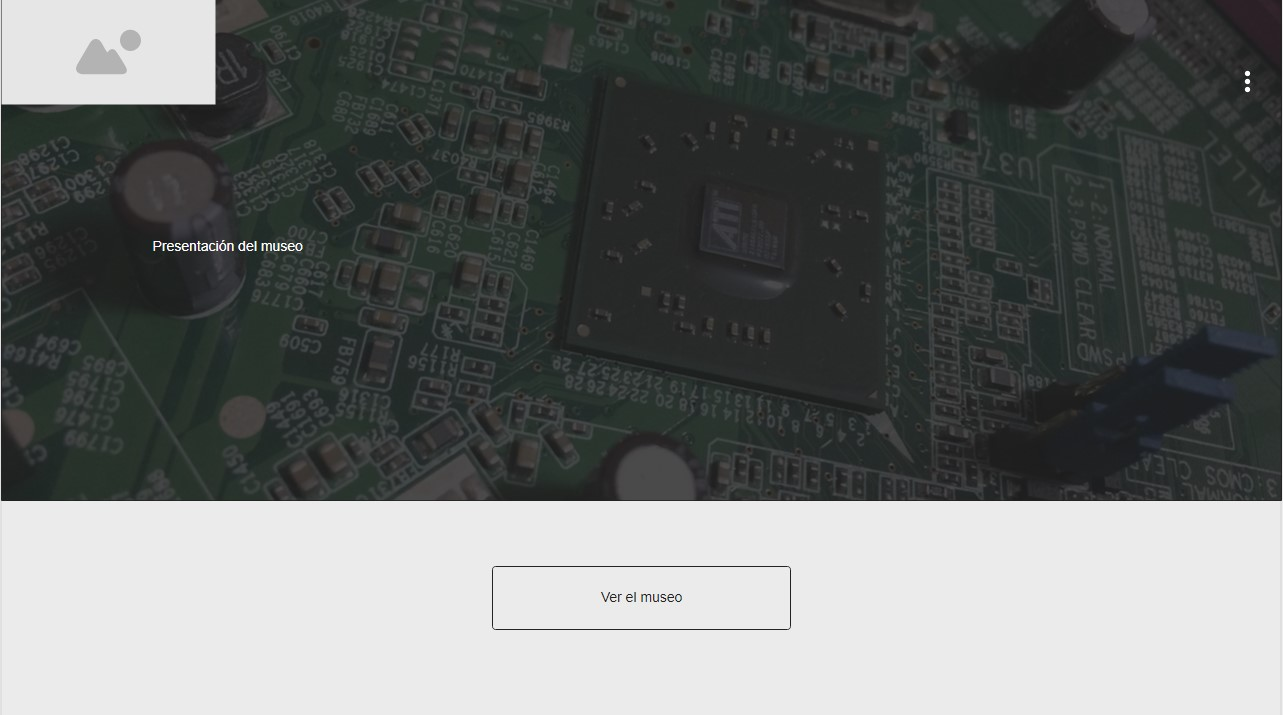
\includegraphics[scale=0.45]{homeIU}
\caption{Prototipo: Página de inicio}
\end{figure}
\paragraph*{Vista general del museo}
\begin{figure}[H]
\centering
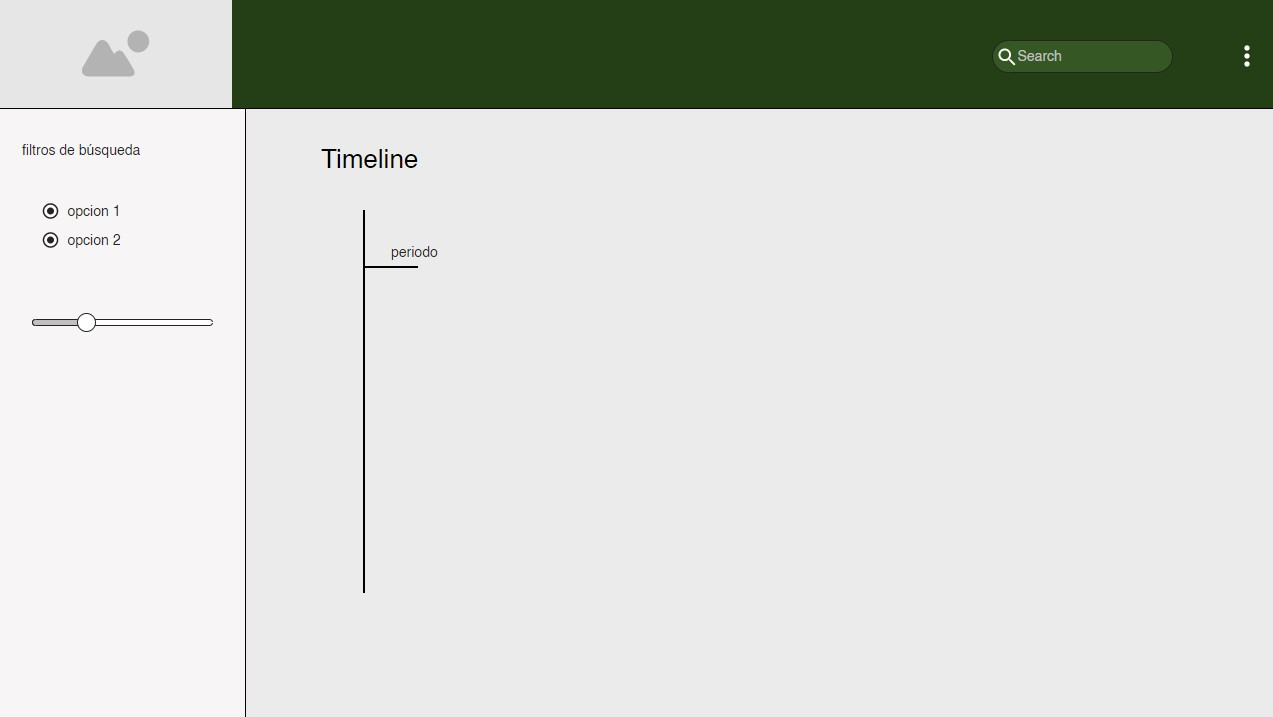
\includegraphics[scale=0.45]{museoIU}
\caption{Prototipo: Vista general del museo}
\end{figure}
\paragraph*{Página de un periodo}
\begin{figure}[H]
\centering
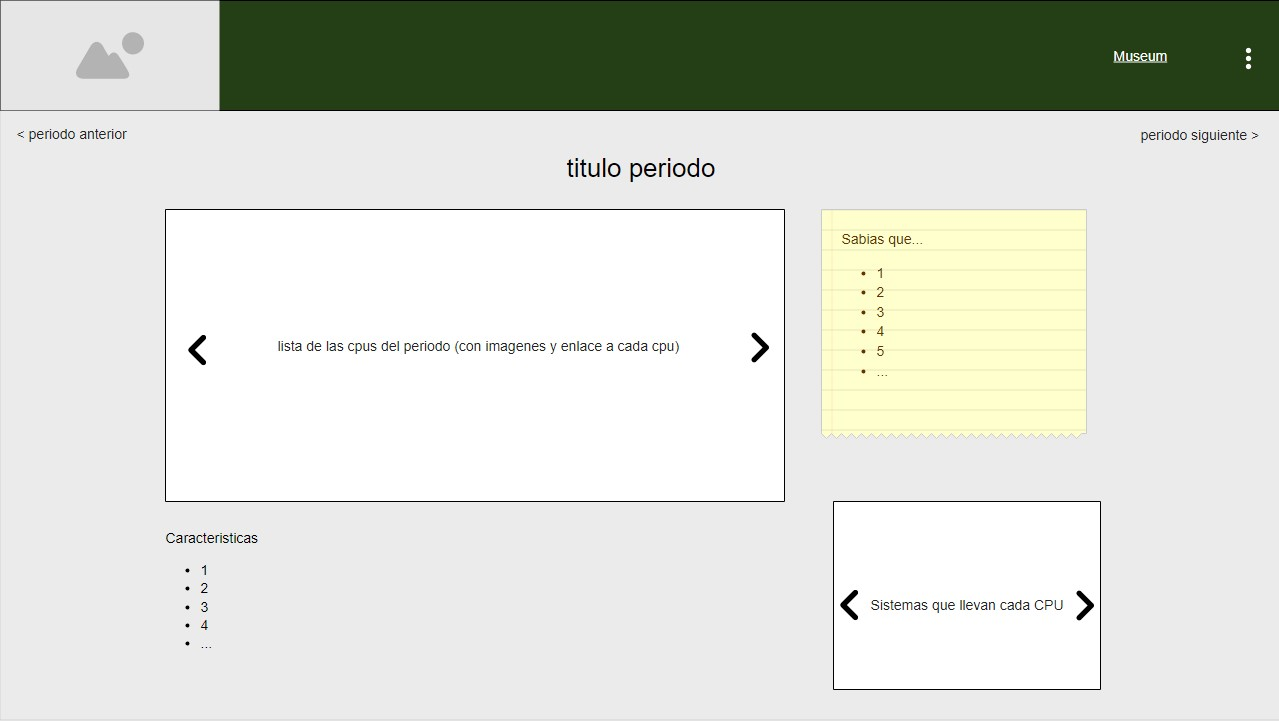
\includegraphics[scale=0.45]{periodoIU}
\caption{Prototipo: Página de un periodo}
\end{figure}
\paragraph*{Página de un componente}
\begin{figure}[H]
\centering
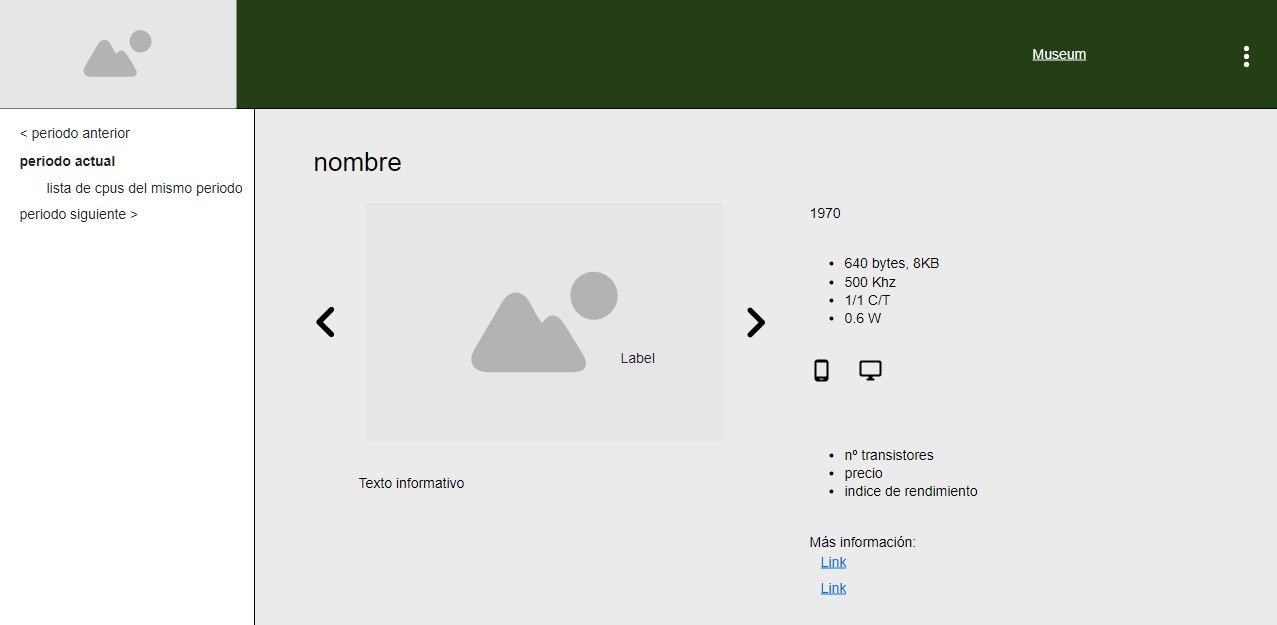
\includegraphics[scale=0.45]{piezaIU}
\caption{Prototipo: Página de un componente}
\end{figure}

\subsection{Definición del aspecto de la interfaz}

\subsection{Descripción del Comportamiento de la Interfaz} 

\subsection{Diagrama de Navegabilidad}


\newpage
\section{ASI 10: ESPECIFICACIÓN DEL PLAN DE PRUEBAS}


\newpage
\chapter{DISEÑO DEL SISTEMA DE INFORMACIÓN}
	\vspace{2cm}	
	\begin{center}
	{\Large \textbf{FASE DE DESARROLLO} \par}
	\end{center}
	\vspace{5cm}
	
	\begin{center}
	\Huge \textbf{DSI}\par
	\end{center}

\newpage


\section{DSI 3: DISEÑO DE CASOS DE USO REALES}

\subsection{Caso de Uso 1.1} 

\subsubsection{Diagramas de Interacción (Comunicación y Secuencia)} 

\subsubsection{Diagramas de Estados de las Clases} 
 
\subsubsection{Diagramas de Actividades} 


\subsection{Caso de Uso 1.2}


\newpage
\section{DSI 4: DISEÑO DE CLASES}

\subsection{Diagrama de Clases}


\newpage
\section{DSI 5: DISEÑO DE LA ARQUITECTURA DE MÓDULOS DEL SISTEMA}

\subsection{DSI 5.1 Diseño de Módulos del Sistema}

\subsection{DSI 5.2 Diseño de Comunicaciones entre Módulos}

\subsection{DSI 5.3 Revisión de la Interfaz de Usuario}


\newpage
\section{DSI 6: DISEÑO FÍSICO DE DATOS}

\subsection{Descripción del SGBD Usado} 
Se ha creado una base de datos relacional, utilizando MySQL 8 como sistema gestor de bases de datos, debido a su gran popularidad en todo el mundo y, más concretamente, en entornos de desarrollo web.\\
\par {\color{red}explicar algo más}

\subsection{Integración del SGBD en Nuestro Sistema} 

\subsection{Diagrama E--R} 


\newpage
\section{DSI 9: DISEÑO DE LA MIGRACIÓN Y CARGA INICIAL DE DATOS}


\newpage
\section{DSI 10: ESPECIFICACIÓN TÉCNICA DEL PLAN DE PRUEBAS}

\subsection{Pruebas Unitarias} 

\subsection{Pruebas de Integración y del Sistema} 

\subsection{Pruebas de Usabilidad y Accesibilidad} 

\subsubsection{Diseño de Cuestionarios} 

\subsubsection{Actividades de las Pruebas de Usabilidad} 


\subsection{Pruebas de Accesibilidad} 

\subsection{Pruebas de Rendimiento} 


\newpage
\chapter{CONSTRUCCIÓN DEL SISTEMA DE INFORMACIÓN}
	\vspace{2cm}	
	\begin{center}
	{\Large \textbf{FASE DE DESARROLLO} \par}
	\end{center}
	\vspace{5cm}
	
	\begin{center}
	\Huge \textbf{CSI}\par
	\end{center}

\newpage


\section{CSI 1: PREPARACIÓN DEL ENTORNO DE GENERACIÓN Y CONSTRUCCIÓN}

\subsection{Estándares y normas seguidos}


\subsection{Lenguajes de programación}


\subsection{Herramientas y programas usados para el desarrollo}


\newpage
\section{CSI 2: GENERACIÓN DEL CÓDIGO DE LOS COMPONENTES Y PROCEDIMIENTOS}

\textcolor[rgb]{0.65,0.16,0}{Ejemplos de tablas descripción de clases}

\begin{table}[H]
\vspace{-4mm}
  \centering
  \caption{Descripción de diseño de LoginScreen}
    \begin{tabular}{p{8.645em}rr}
    \toprule
    \rowcolor[rgb]{ .851,  .886,  .953} \multicolumn{3}{p{31.285em}}{\textbf{LoginScreen}} \\
    \midrule
    \rowcolor[rgb]{ .949,  .949,  .949} \multicolumn{3}{p{31.285em}}{\textbf{Descripción}} \\
    \midrule
    \multicolumn{3}{p{31.285em}}{Es la encargada de las acciones y la renderización de la pantalla de inicio de sesión.} \\
    \midrule
    \rowcolor[rgb]{ .906,  .902,  .902} \multicolumn{3}{p{31.285em}}{\textbf{Atributos propuestos}} \\
    \midrule
    \multicolumn{3}{p{31.285em}}{-} \\
    \midrule
    \rowcolor[rgb]{ .906,  .902,  .902} \multicolumn{3}{p{31.285em}}{\textbf{Métodos propuestos}} \\
    \midrule
    \textbf{signInWithGoogle} & \multicolumn{2}{p{22.64em}}{Hace una llamada al objeto Fire para el inicio de sesión con Firebase authentication mediante una cuenta de Google.} \\
    \midrule
    \textbf{render} & \multicolumn{2}{r}{} \\
    \bottomrule
    \end{tabular}%
\end{table}%


\begin{table}[htbp]
  \centering
  \caption{Descripción de diseño de HomeScreen}
    \begin{tabular}{p{10em}rr}
    \toprule
    \rowcolor[rgb]{ .851,  .886,  .953} \multicolumn{3}{p{31.285em}}{\textbf{HomeScreen}} \\
    \midrule
    \rowcolor[rgb]{ .949,  .949,  .949} \multicolumn{3}{p{31.285em}}{\textbf{Descripción}} \\
    \midrule
    \multicolumn{3}{p{31.285em}}{Es la encargada de las acciones y la renderización de la pantalla de emergencia.} \\
    \midrule
    \rowcolor[rgb]{ .906,  .902,  .902} \multicolumn{3}{p{31.285em}}{\textbf{Atributos propuestos}} \\
    \midrule
    \multicolumn{3}{p{31.285em}}{-} \\
    \midrule
    \rowcolor[rgb]{ .906,  .902,  .902} \multicolumn{3}{p{31.285em}}{\textbf{Métodos propuestos}} \\
    \midrule
    \textbf{componentWillMount} & \multicolumn{2}{r}{} \\
    \midrule
    \textbf{emergencyCalling} & \multicolumn{2}{p{21.285em}}{Es el método encargado de redirigir la aplicación hacia el marcador con el 112 marcado.} \\
    \midrule
    \textbf{warnProtectors} & \multicolumn{2}{p{21.285em}}{[Falta implementar] Es el encargado de generar un mensaje de aviso a los protectores creando notificaciones push.} \\
    \midrule
    \textbf{render} & \multicolumn{2}{r}{} \\
    \bottomrule
    \end{tabular}%
\end{table}%

\newpage
\section{CSI 3: EJECUCIÓN DE LAS PRUEBAS UNITARIAS}


\newpage
\section{CSI 4: EJECUCIÓN DE LAS PRUEBAS DE INTEGRACIÓN}


\newpage
\section{CSI 5: EJECUCIÓN DE LAS PRUEBAS DEL SISTEMA}

\subsection{Prueba de Usabilidad}

\subsection{Pruebas de Accesibilidad} 
 
\subsubsection{Revisión Preliminar} 

\subsubsection{Evaluación de Conformidad} 

\subsubsection{Checklist del WCAG 2.1} 

\subsubsection{Accesibilidad con Dispositivos Móviles} 


\newpage
\section{CSI 6: ELABORACIÓN DE LOS MANUALES DE USUARIO}

\subsection{Manual de Instalación} 

\subsection{Manual de Ejecución} 

\subsection{Manual de Usuario} 

\subsection{Manual del Programador}


\newpage
\section{CSI 8: CONSTRUCCIÓN DE LOS COMPONENTES Y PROCEDIMIENTOS DE MIGRACIÓN Y CARGA INICIAL DE DATOS}



\newpage
\chapter{IMPLANTACIÓN Y ACEPTACIÓN DEL SISTEMA}
	\vspace{2cm}	
	\begin{center}
	{\Large \textbf{FASE DE DESARROLLO} \par}
	\end{center}
	\vspace{5cm}
	
	\begin{center}
	\Huge \textbf{IAS}\par
	\end{center}

\newpage

\section{IAS 1: ESTABLECIMIENTO DEL PLAN DE IMPLANTACIÓN}


\newpage
\section{IAS 4: CARGA DE DATOS AL ENTORNO DE OPERACIÓN}


\newpage
\section{IAS 5: PRUEBAS DE IMPLANTACIÓN DEL SISTEMA}


\newpage
\section{IAS 7: PREPARACIÓN DEL MANTENIMIENTO DEL SISTEMA}


\newpage
\section{IAS 8: ESTABLECIMIENTO DEL ACUERDO DE NIVEL DE SERVICIO}


\newpage
\section{IAS 9--10: PRESENTACIÓN Y APROBACIÓN DEL SISTEMA Y PASO A PRODUCCIÓN}


\newpage
\chapter{CONCLUSIONES Y AMPLIACIONES}
\newpage

\section{CONCLUSIONES}

\newpage
\section{AMPLIACIONES} 


\newpage
\chapter*{ANEXOS}
\addcontentsline{toc}{chapter}{ANEXOS}
\newpage
\phantomsection
\section*{PLAN DE GESTIÓN DE RIESGOS}
\addcontentsline{toc}{section}{PLAN DE GESTIÓN DE RIESGOS}

\newpage
\section*{CONTENIDO ENTREGADO EN LOS ANEXOS} 
\addcontentsline{toc}{section}{CONTENIDO ENTREGADO EN LOS ANEXOS}

\subsection*{Contenidos} 

\textcolor[rgb]{0.65,0.16,0}{Ejemplo de como especificar los contenidos entregados}

Además de este documento, se hace entrega de una carpeta comprimida ``.zip'' en la que ahora se describirán sus contenidos. Se estructurará también la organización del código fuente.

\begin{itemize}
	\item \textbf{Planificación\_TFG.mpp} -> Archivo de Microsoft Project que contiene la planificación del proyecto entera.
	\item \textbf{Presupuesto-GuardMe\_TFG.xlsx} -> Archivo Microsoft Excel que contiene los cálculos del presupuesto del proyecto.
	\item \textbf{Diagramas} -> Carpeta que contiene todos los diagramas utilizados en este documento.
	\begin{itemize}
		\item \textit{Diagrama\_de\_paquetes.png}
		\item \textit{Diagrama\_firestore.png}
		\item \textit{Diagrama\_navegabilidad.png}
		\item \textit{Diagrama\_secuencia\_enviar.png}
		\item \textit{Diagrama\_secuencia\_visualizar.png}
		\item \textit{Diagrama\_UML-Diseño.png}
		\item \textit{Diagrama\_UML-Analisis.png}
	\end{itemize}
	\item \textbf{TFG\_codigo.zip} -> Carpeta comprimida con todo el código fuente.
\end{itemize}

Ahora se mostrará el contenido de dicha carpeta comprimida que contiene todo el código fuente de la aplicación la cual esta dividida a su vez en dos carpetas:

\paragraph*{AuthServerGuardMe}
Contiene el código que se aloja en \textit{Heroku} para darle funcionalidad al servidor. La clase principal es la llamada \texttt{mainAuthServer.js}.

\paragraph*{GuardMe}
Contiene el código fuente de la aplicación y se compone de las siguientes carpetas:
\begin{itemize}
	\item \textbf{assets} -> Carpeta que contiene los elementos gráficos usados en la aplicación. Se subdivide en una carpeta llamada \textit{images} que contiene todas las imagenes utilizadas para la construcción de la aplicación.
	\item \textbf{components} -> Carpeta que contiene el código para todos los componentes creados.
	\item \textbf{constants} -> Carpeta que contiene el código
	\item \textbf{docs} -> Carpeta que contiene los archivos html generados por JSDoc.
	\item \textbf{files} -> Carpeta en la que se encuentras los futuros archivos de Términos y Condiciones y Política de Privacidad entre otros.
	\item \textbf{modules\_LICENSES} -> Carpeta que contiene una por una todas las licencias de las librerías utilizadas en el desarrollo.
	\item \textbf{navigation} -> Carpeta que contiene las clases relativas a la navegación de la aplicación.
	\item \textbf{objects} -> Carpeta que contiene los objetos utilizados en el desarrollo que en este caso ha sido solo Fire.js.
	\item \textbf{screens} -> Carpeta que contiene todas las pantallas, agrupadas a su vez en subcarpetas que identifican la pantalla sobre la que están relacionadas.
	\item \textbf{styles} -> Carpeta que contiene todos los estilos de las pantallas, agrupadas a su vez en subcarpetas que siguen la misma estructura que \textit{screens}.
	\item \textbf{App.js} -> Clase principal y encargada de que comience la aplicación entera.
	\item \textbf{LICENSE} -> Licencia sobre el código fuente.
	\item \textbf{README.md} -> Archivo con la descripción del proyecto para la documentación y el repositorio de GitHub.
	\item \textbf{package.json} -> Archivo que contiene las librerías utilizadas en el proyecto.
	\item \textbf{app.json} -> Archivo que contiene la configuración de la aplicación.
	\item \textbf{configJSDoc.json} -> Archivo de configuración para la creación de documentación por parte de JSDoc.
	\item \textbf{Otros archivos} -> Los demás archivos no son relevantes ya que muchos se generan por defecto y los demás son configuraciones propias de expo.
\end{itemize}

\newpage
\nocite{*} %El comando bibliography enseña solo las referencias que se hayan usado en el texto. Este comando permite "no citar" todas y así que aparezcan.
\bibliographystyle{ieeetr} 
\bibliography{references}

\newpage





\end{document}
